\documentclass[a4paper, 11pt]{article}

\usepackage[british]{babel}
\usepackage[autostyle]{csquotes}
% \usepackage[colorlinks=true, urlcolor=blue, citecolor=blue, linkcolor=blue]{hyperref}
\usepackage[hidelinks]{hyperref}
\usepackage{graphicx}
\usepackage{float}
\usepackage{geometry}
\usepackage[toc,page]{appendix}
\usepackage{caption}
\usepackage{subcaption}

\graphicspath{{images/}}
\geometry{margin=2.0cm}

\begin{document}

\title{Machine Learning to Study Patterns in Chess Games}
\author{Student Number: 690065435}
\date{Academic Year 2022/2023}

\maketitle

\begin{abstract}
{Abstract here}.

\begin{center}
\end{center}
\end{abstract}

\vspace*{\fill}
\begin{center}

\vspace{1em}
I certify that all material in this report which is not my own work has been identified.
\end{center}
\vspace{1em}

Signature: \hrulefill

\newpage
\tableofcontents
\newpage

\section{Introduction}
Chess is one of the oldest and most popular board games globally -- it has a rich history and vast literature dating back centuries, with the first comprehensive book about chess called \textquote{Book of the Chess} appearing in the year 840, discussing chess openings, endings, and hundreds of chess problems \cite{earliestChessBooks,wonning2014short}. However, the large-scale exploration of chess games has only caught on recently -- the most well-known and highest-rated chess engine \cite{computerChessRatingLists}, Stockfish, has used over 9,400 years of CPU time to analyse over 5.6 billion self-play chess games as of April 2023 \cite{stockfishTestingFramework}. Websites such as Lichess and Chess.com have provided an online platform for people to play chess -- users can create a free account and search for a game with other players with various time controls, where their matchmaking system will pair them with a player of a similar skill level. These platforms have made the game accessible to more people in standardised formats -- this has enabled the collection of data on a large scale, which makes it a fascinating domain for data mining and machine learning. Furthermore, chess games involve cognition and human behaviour that we can apply more generally -- there have been studies in areas like social learning theory on other games such as Go \cite{beheim2014strategic}, but they also apply to chess.

In this dissertation, we explore data mining and machine learning techniques to analyse large-scale data from the Lichess Open Database, which contains monthly records on tens of millions of chess games played by users of various skill levels. Our goal is to discover patterns and insights into how people play chess, which could contribute to further studies in chess such as cheat detection algorithms to improve the integrity of chess tournaments and promote positive growth in the game.

\section{Preliminary Research}

\subsection{Early History of Computer Chess}
Since the first digital computer switched on in 1945, programmers have been interested in using computers to play chess. In 1948, Alan Turing worked with David Champnowne to create the \textquote{Turochamp}, a machine routine for playing chess \cite{copeland2005turing}. Claude Shannon wrote a paper in 1949 describing a computer that could play chess by analysing the seven most likely moves from the current positions and branching these into the seven most likely replies from the opposition continuously until the computer ran out of memory \cite{shannon1950xxii}. Dietrich Prinz eventually implemented the first chess program in November 1951, though it could not complete an entire chess game, and it used exhaustive search to play moves rather than a heuristic \cite{copeland2005turing}.

IBM made a significant breakthrough with their Deep Blue supercomputer starting with their initial prototype in 1995 \cite{hsu1995deep}. It was released in 1996 \cite{hsu1999ibm} and was able to perform 200 million calculations per second \cite{strogatz2018one}. Deep Blue was the first computer to use a heuristic search algorithm, searching for a solution to a problem by evaluating possible solutions and choosing the best one. In 1997, Deep Blue became the first computer to beat a world champion as it defeated Garry Kasparov over a six-game match \cite{seirawan1997implications}, indicating that chess engines were better than human players. However, a lack of a deep understanding of the game was evident -- Deep Blue accepted Kasparov's sacrifice of a rook for a bishop in the first game, only to lose 16 moves later \cite{strogatz2018one}.

\subsection{Modern Developments in Computer Chess}
Stockfish is the strongest chess engine in the world. Both Lichess and Chess.com use Stockfish to provide game analysis on their platforms, and it is also used by professional players to analyse their games. It was released as a free, open-source chess engine in November 2008 \cite{aboutStockfish}, with volunteers donating CPU time to test improvements to the engine using a distributed framework, Fishtest \cite{fishtestDistributedTestingFramework}. Stockfish uses the alpha-beta pruning search algorithm which improves minimax search \cite{v1928theorie} by avoiding variations that will never be reached in optimal play due to either player redirecting the game \cite{maharaj2022chess}.

However, other chess engines have used different algorithms in recent history. Most notably, DeepMind released AlphaZero in 2017 \cite{silver2017mastering2} based solely on reinforcement learning -- it had no knowledge of chess beyond the basic rules and learned within hours by playing millions of games \cite{strogatz2018one}. AlphaZero used a general-purpose Monte Carlo tree search algorithm, a heuristic search algorithm \cite{silver2017mastering2}. It uses a tree to represent the game state, then randomly selects moves and uses the results of each game to weigh the tree nodes accordingly \cite{chaslot2008monte}. In December 2017, AlphaZero beat Stockfish in a 100-game match with 28 wins, 72 draws, and zero losses \cite{klein2017google}, showing the feasibility of alternative approaches, although Stockfish has since improved.

These developments in computer chess demonstrate the potential of big data in chess. While chess engines have gathered a lot of attention from researchers, there has been less attention paid to patterns and insights into how people play chess, which is what our project will focus on.

\subsection{Growth in the Popularity of Chess}
Chess has seen a resurgence in popularity over the last decade. The rise of chess platforms such as Lichess and Chess.com have enabled people to play chess games online with other people globally in seconds. Lichess recorded 121,332 standard-rated games in January 2013, which rose to 103,178,407 games a decade later in January 2023 \cite{lichessOpenDatabase}. 

More recently, popular culture has driven a chess boom. As the COVID-19 pandemic struck in late 2019, people turned to chess to fill their spare time. The release of The Queen's Gambit in October 2020 accelerated people's interest -- Netflix announced that a then-record 62 million households watched the series in its first 28 days \cite{chessIsBooming}. Chess.com saw its monthly active users double from around 8 million to nearly 17 million between October 2020 and April 2022 \cite{chessIsBooming}. It also reported a record for the monthly number of chess games played, with 1 billion games played in February 2023 \cite{chessCom1BillionGamesInFebruary}. Chess was also featured in the most popular social media post in 2022, featuring Cristiano Ronaldo (the most followed user on Instagram) playing chess with Lionel Messi on an Instagram post that has received over 42,800,000 likes as of April 2023 \cite{ronaldoMessiChess}.

The fast growth of chess has given us increasing amounts of and better quality data to analyse, which is critical to the success of our project. As previously mentioned, Lichess records tens of millions of games every month, and they make this accessible to the public through their Open Database \cite{lichessOpenDatabase}, which is what our project will use as its data source.

\subsection{Practical Uses of Chess Databases}

\section{Project Specification}
I will be investigating the following question: can we use data mining and machine learning techniques on historical data to discover patterns and insights in how people play chess? Our project will be broken down into the following objectives:

\begin{itemize}
    % \setlength\itemsep{-0.5em}
    \setlength\itemsep{0em}
    \item Create a data pipeline for downloading and processing the data efficiently
    \item Explore the data to find interesting patterns and insights
    \item Implement machine learning to create models based on patterns in chess games
    \item Analyse and evaluate the usefulness of the models
\end{itemize}

In the next section, we will discuss how we will achieve these objectives by downloading the data, processing it, and analysing it.

\section{Design, Methods, and Implementation}

\subsection{Downloading the Data}
Collecting the data correctly was paramount to the success of our project, and it was important to use a large sample size to ensure that our insights represent the general population of chess games. We used the Lichess Open Database \cite{lichessOpenDatabase} of standard rated games for our data source -- they upload tens of millions of games every month in PGN format, and they are easily accessible to the public. We decided to focus on games in 2022, as this enables me to capture the latest trends in chess.

The time controls in Lichess are decided based on the estimated game duration, using the formula: $total \; time \; in \; seconds = (initial \; clock \; time) + 40 \times (clock \; increment)$. Games between 29 seconds and 179 seconds are Bullet; games between 179 seconds and 479 seconds are Blitz, games between 479 seconds and 1499 seconds are Rapid, and games over 1500 seconds are Classical. Furthermore, games are either Rated or Unrated -- the former results in rating points changing based on the game outcome, whereas the latter does not. The Lichess Open Database only includes Rated games. We will only be analysing Rated Bullet, Rated Blitz, and Rated Rapid games -- we will not be including Rated Classical games, as they have a significantly smaller sample size and the longer time controls result in a vastly different playstyle.

We started by downloading the PGN files for each month, which introduced difficulties with big data. Each month's file is around 30 GB to download and they are compressed, which means each month is around 210 GB when uncompressed, resulting in approximately 2.5 TB of data for the year. My laptop only had 1 TB of storage, and the sheer size of the data would make it unrealistic to process in a reasonable amount of time. Therefore, we collected a sample of 6 million chess games from each month which we would later filter down.

\subsection{Data Processing}
PGN (Portable Game Notation) files are a standard format for recording chess games -- each game has headers containing information like the white player, black player, their ratings, and the result of the game. In addition, it stores a list of all the moves in each game. While PGN files are well-structured, they are not easy to process. The pgn2data Python library \cite{pgn2dataGitHub} provides a simple way to convert PGN files into CSV files, but it exported both the moves and the metadata of each game in separate CSV files. We did not need the moves, so it was using up unnecessary space and taking a long time to process each game. It was also designed for generic PGN files so it did not include additional useful metadata provided by Lichess such as the opening of the game.

Thus, we wrote our own Python script to convert each PGN file into a single CSV file containing only the metadata of each game. We used the python-chess library to parse the PGN files and iterate over each game, skipping Rated Bullet games, Rated Classical games, games that involved a non-human player, and games that were abandoned. Our sample reduced from 60 million games to slightly over 40 million games after filtering it. To optimise performance, we split each month's PGN into six files each containing 1 million games with pgn-extract (a PGN manipulator written in C) \cite{pgnExtractGitHub}, and we used Python's multiprocessing library to process each month in parallel -- this reduced the processing time from 120 minutes to 20 minutes for each month on my Apple M1 Max chip.

Once we had a CSV for each month, we combined them into a single CSV file containing our final data set. We converted this CSV to a folder of Parquet files using Dask \cite{dask}, which is a library for parallel computing in Python and extends common interfaces like pandas \cite{pandas} to handle big data in a larger-than-memory environment. This significantly reduced the load time for the data, and it meant we could use the Dask library to perform parallel computations on the data.

For low-level, turn-based analysis of games, we created a .scout file using Scoutfish (a tool for querying chess databases written with C++) \cite{scoutfish} to enable fast queries. For example, we can query the database to find all games where the board state is a certain position using the FEN (Forsyth-Edwards Notation) of the position, which is the standard string used in chess to represent the board state -- this may be useful for finding occurrences of a specific variation of an opening. It provides the offset line number of each matching game in the PGN file, which we can use to find more information about the game. However, Scoutfish queries are not intuitive to write, so it can take a lot of effort to get insights using this tool. Therefore, we will primarily focus on high-level analysis of game metadata using Dask DataFrames.

\begin{figure}[H]
    \centering
    \caption{Diagram of the Data Pipeline}
    \label{fig:dataPipeline}
    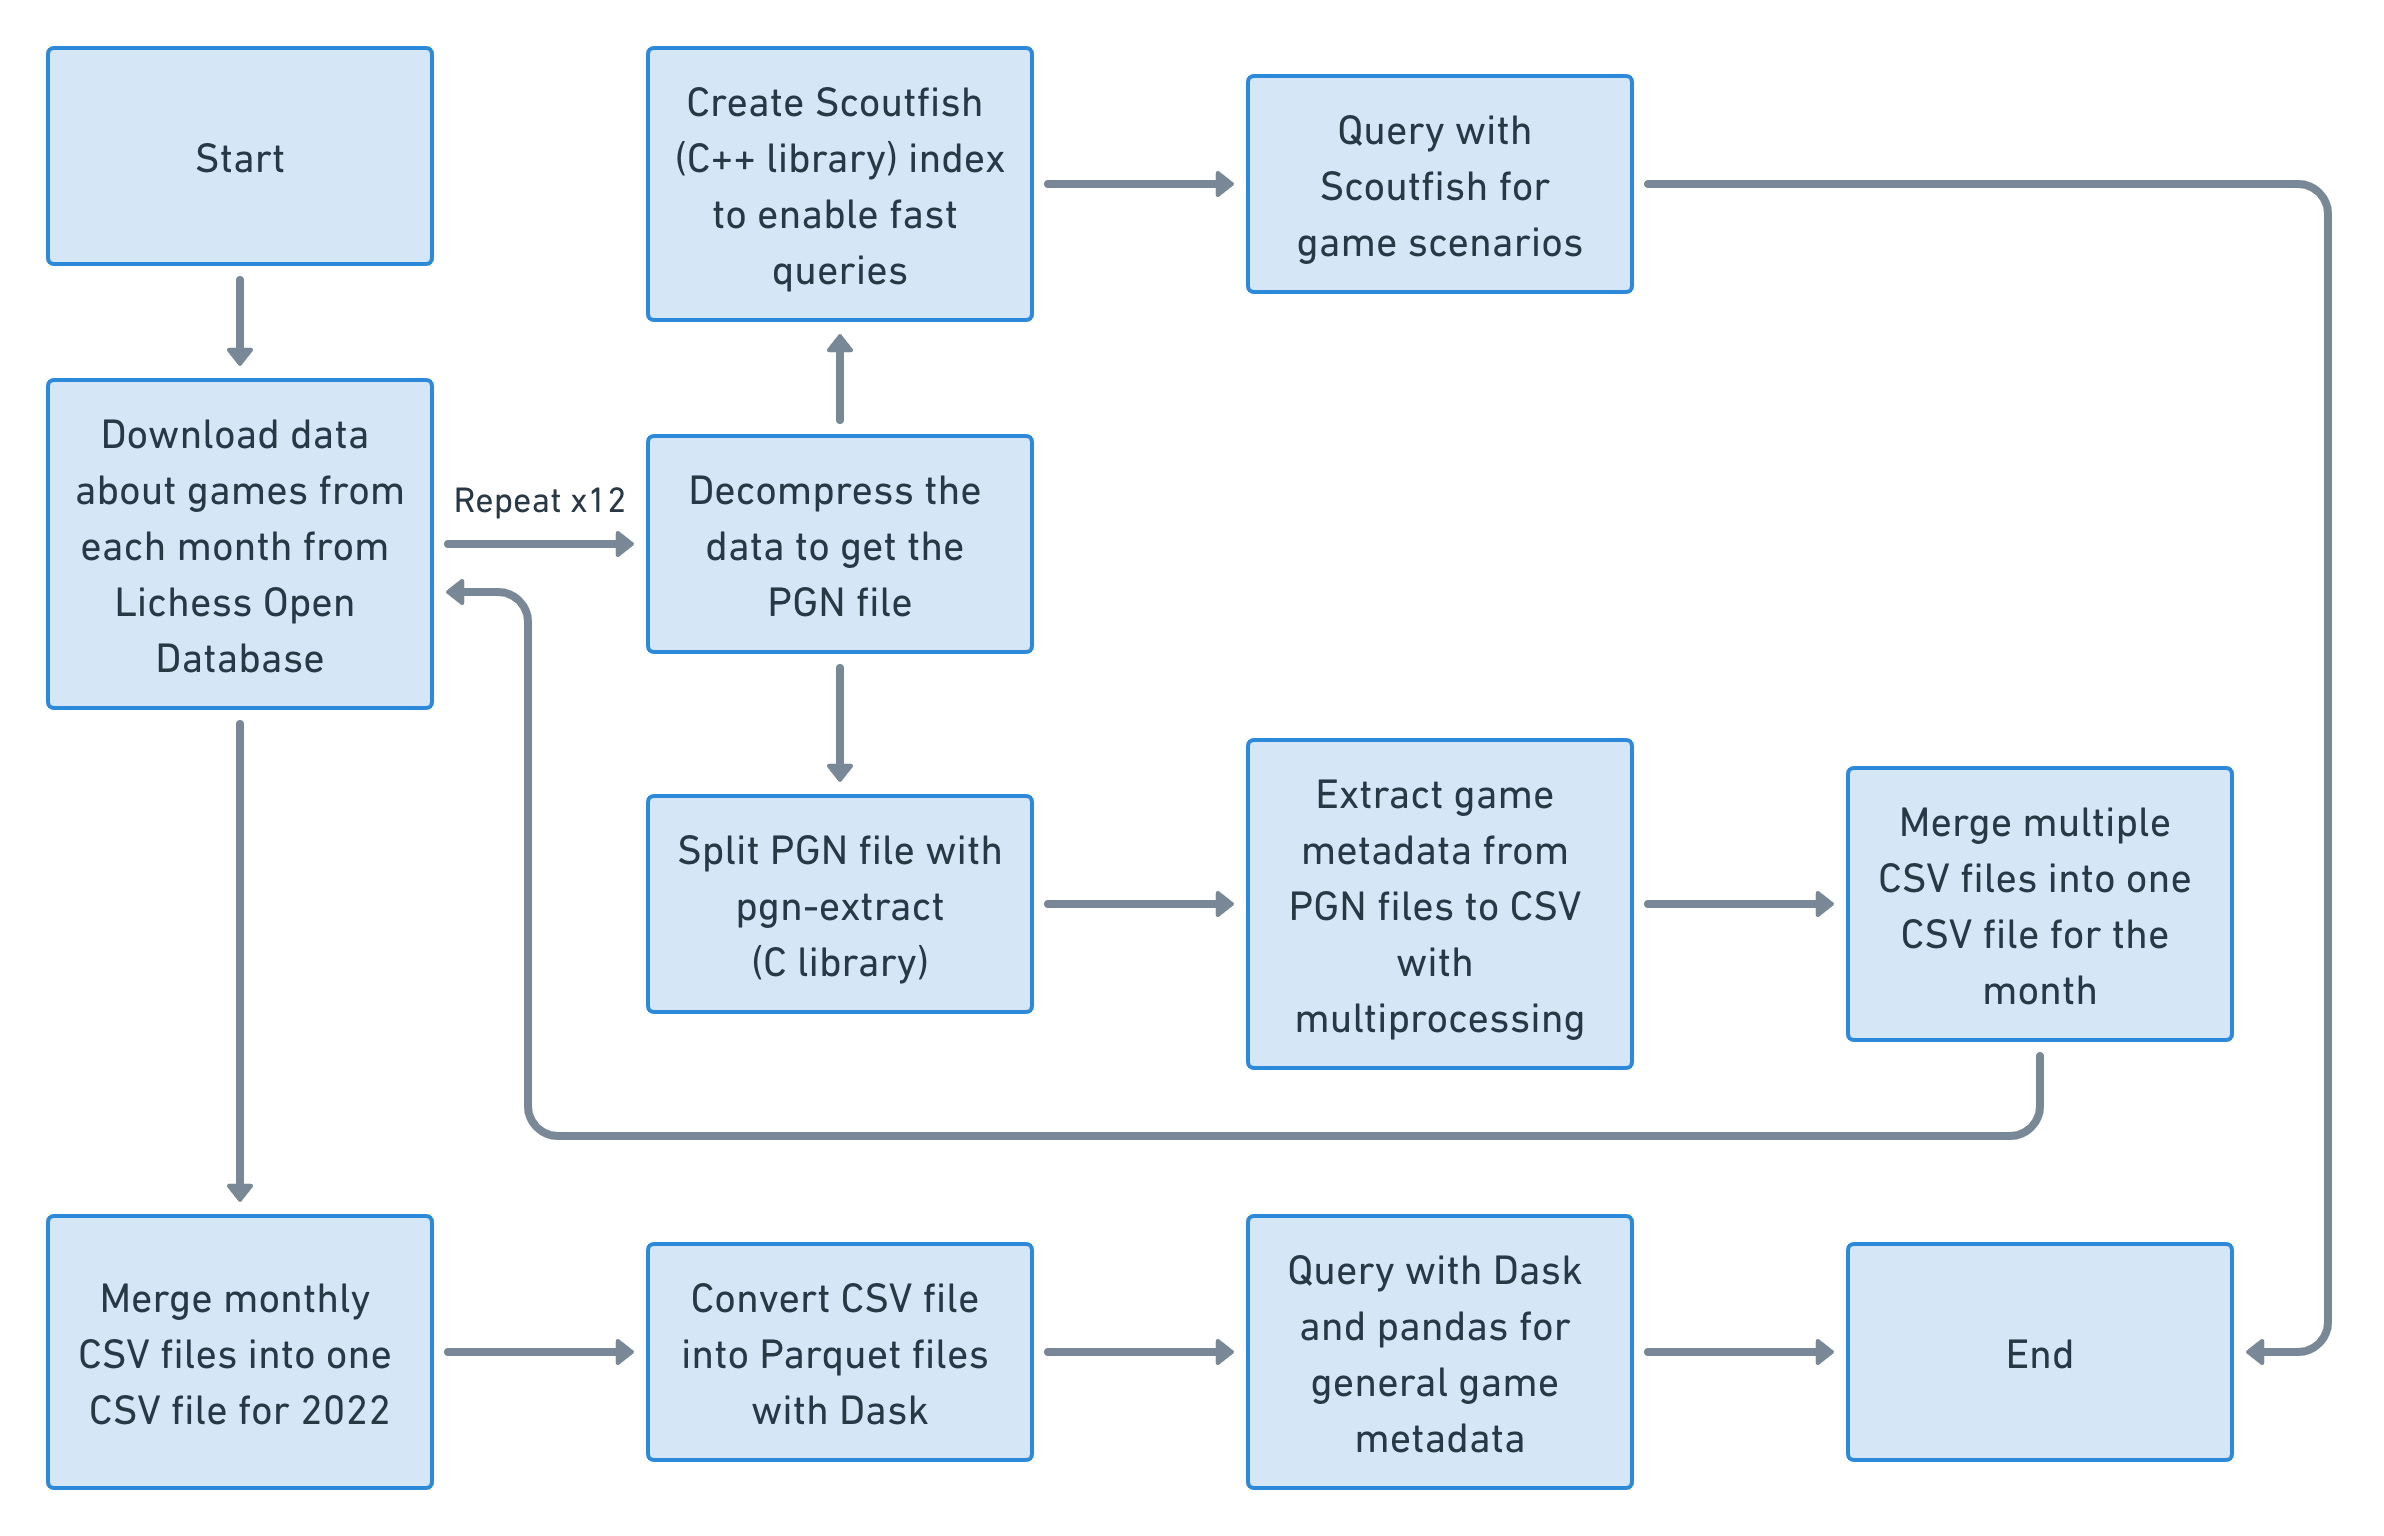
\includegraphics[width=0.8\textwidth]{Data Pipeline.png}
\end{figure}

Figure \ref{fig:dataPipeline} shows an overview of our data pipeline. It shows how we used the Lichess Open Database to collect the data over 12 months. To analyse game metadata, we aggregated the data into a single CSV file, and converted it to a folder of Parquet files to query with Dask. Meanwhile, to perform more detailed analysis of game scenarios, we used this data to create a Scout index to enable fast queries.

We also created a Python script to convert the CSV file to an SQLite3 database -- this enables us to perform queries on the data over SQL for manual data exploration, which is easier and more interactive than using Dask functions.

\section{Data Exploration}

\subsection{Structure of Data}
Our data consists of 40,121,728 Rated Blitz and Rated Rapid games that were played on Lichess in 2022. Each game is described by: the datetime of when the game started, what type of game (Rated Blitz or Rapid) it was, the specific time control, outcome of the game (1-0 for a White win, 1/2-1/2 for a draw, and 0-1 for a Black win), how the game ended, ECO category of the opening, the specific opening that was played, who played White and Black, their Lichess ratings, and a URL to the game on Lichess. Figure \ref{fig:structureOfData} shows the head of the DataFrame, which contains the first five games in the data sample.

\begin{figure}[H]
    \centering
    \caption{Structure of Data}
    \label{fig:structureOfData}
    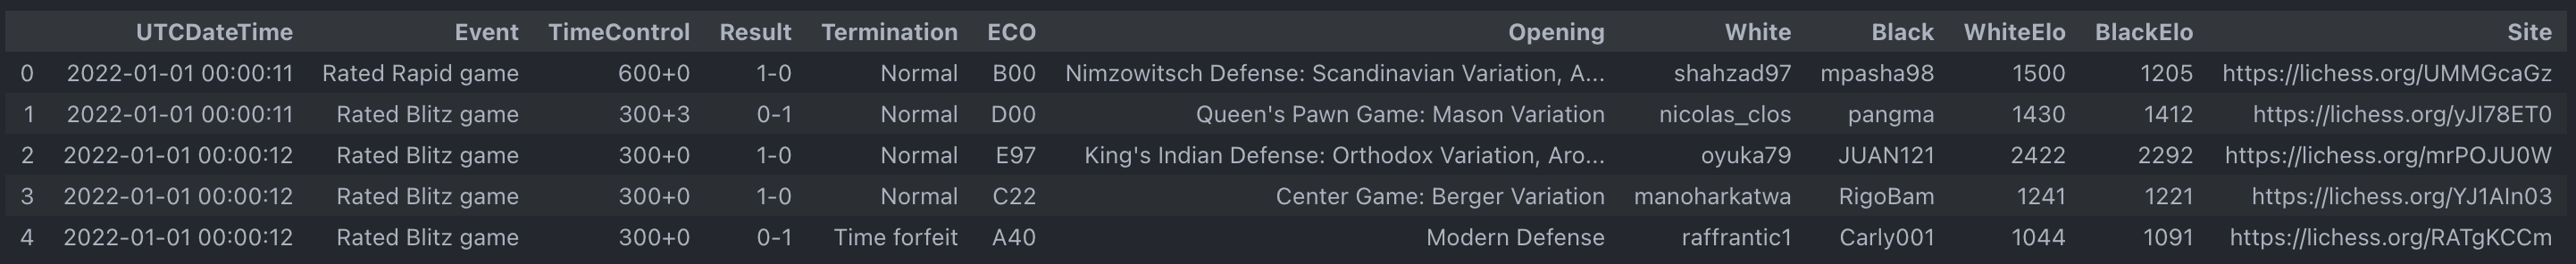
\includegraphics[width=\textwidth]{Structure of Data.png}
\end{figure}

\subsection{Distribution of Player Ratings}
We counted the ratings of players in our data set. Rating systems are designed to predict the outcome of games so that players can be matched fairly. There are various rating systems used in chess -- the most common is the Elo rating system, which is used by various sports. Lichess uses the Glicko 2 rating system, which accounts for volatility amongst other factors to provide better prediction accuracy than the Glicko 1 and Elo rating systems \cite{chessRatingSystems, DeloitteFIDEChessRatingChallenge}. The Glicko 2 rating system starts at 1500, and it is artificially limited to a minimum of 600 in Lichess. We created bins of 200 rating point ranges starting from 600 -- this handles the representation of new players well, as those who have played few games will not have changed their rating significantly and likely get placed in the 1400-1600 bin. Note that the last four bins on the right of the bar chart do exist, but they are difficult to see -- they contain totals of 11,622 for 2800-3000, 382 for 3000-3200, 459 for 3200-3400, and 1 player for 3400-3600. In addition, the counts are based on each game played, so some players may be overrepresented in the data set -- a player who plays 100 games within the year will have 100 entries in the data set, whereas a player who plays 1 game will have 1 entry. However, this is not a significant issue because the data set is large enough to represent the distribution of player ratings well.

\begin{figure}[H]
    \centering
    \caption{Distribution of Player Ratings on Lichess in 2022}
    \label{fig:distributionOfPlayerRatings}
    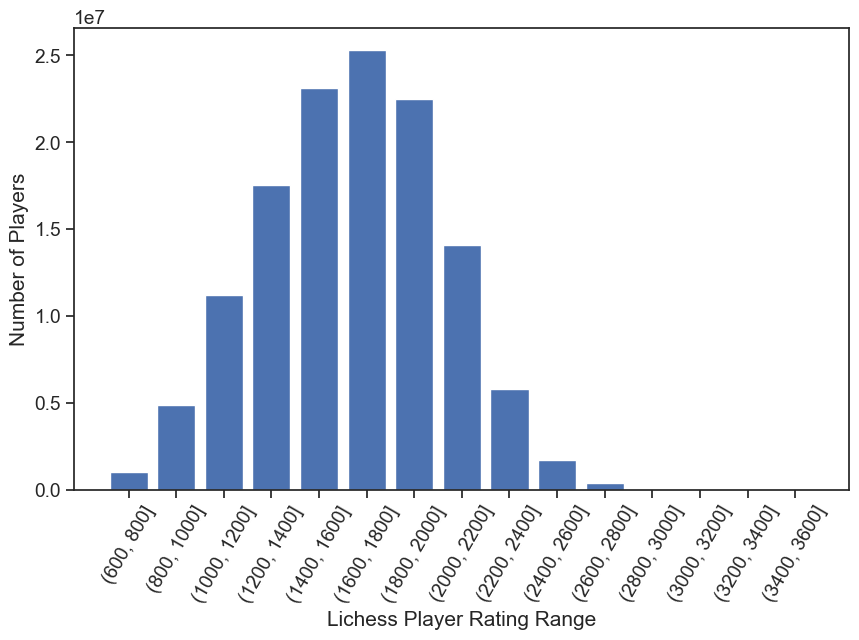
\includegraphics[width=0.8\textwidth]{Distribution of Player Ratings.png}
\end{figure}

Figure \ref{fig:distributionOfPlayerRatings} shows that the distribution of player ratings tends towards a normal distribution. We could explain this based on the concept that a player's performance is similar to a random walk, which states that an object moves randomly with equal probability in different directions. In Lichess ratings, a player's rating can be seen as the result of a series of random walks, where the player's rating constantly changes as they win and lose games. Over time, their rating will tend to stabilise to represent their true skill level. Moreover, the central limit theorem states that the sum of a large number of independent and identically distributed random variables tends towards a normal distribution \cite{le1986central}. In this case, the ratings of individual players can be seen as independent and identically distributed random variables, with each game representing a single trial. Therefore, the central limit theorem predicts that the distribution of ratings will tend towards a normal distribution as the number of games increases. This is supported by how largest bin is the 1400-1600 bin, which contains the starting rating of 1500. Lichess' matchmaking system could contribute to this -- it matches players with similar skill, so games theoretically end up with a roughly equal number of wins and losses.

\subsection{Effect of Rating Differential on Win Rate}
Next, we investigated the impact of player rating differentials on White's win rate. To begin with, we counted the outcomes of all games, and then counted the outcomes of games when White had a higher rating -- White won 49.69\% of all games, which rose to 53.98\% of games when they had a higher rating than their opponent (as shown in figure \ref{fig:effectOfHigherRatingOnWhiteWinRate} from the appendices). Then, we sought to quantify the impact of rating differential in both absolute and relative terms -- the former was the difference in rating between the two players, and the latter was the difference in rating divided by the mean rating of the two players. Figure \ref{fig:distributionOfAbsoluteRatingDifference} and figure \ref{fig:distributionOfRelativeRatingDifference} from the appendices show the distribution of the absolute and relative rating differences. We grouped the data by rating differential and calculated the win rate for White. For example, when White is rated 1100 and Black is rated 900, the absolute rating differential is 200, whereas the relative rating differential is 10\%. We focused on the win rate for White because the opening of the game is usually decided by White.

The results showed that there is a clear positive correlation between rating differential and White's win rate. Both the absolute and relative differential metrics corroborate this, but we saw that relative rating difference highlighted the impact of rating on White's win rate more clearly. Absolute rating differential (shown in figure \ref{fig:meanWhiteWinRateForEachEloDiffBin} from the appendices) is more intuitive to understand, but it is less accurate than relative rating differential (shown in figure \ref{fig:meanWhiteWinRateForEachRelativeEloDiffBin}) because it is not normalised.

\begin{figure}[H]
    \centering
    \caption{Mean White Win Rate for Each RelativeEloDiff Bin}
    \label{fig:meanWhiteWinRateForEachRelativeEloDiffBin}
    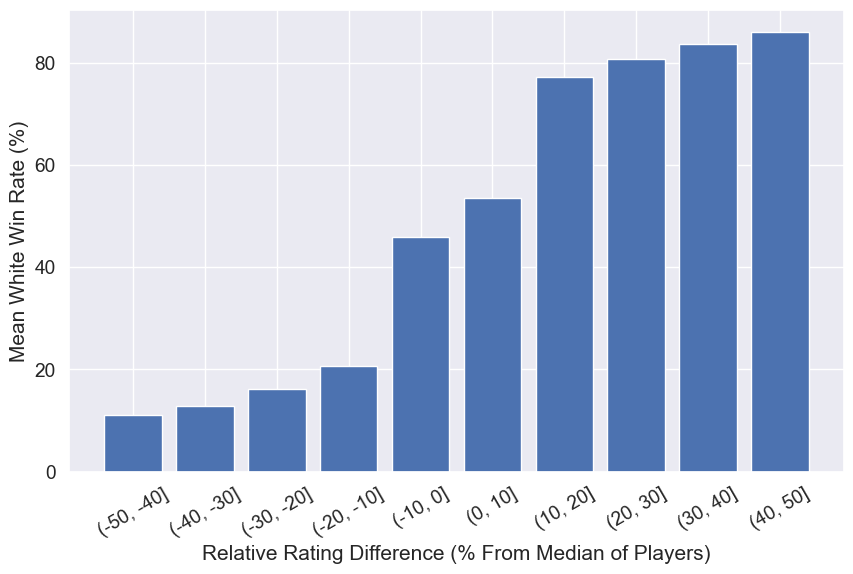
\includegraphics[width=0.8\textwidth]{Mean White Win Rate for Each RelativeEloDiff Bin.png}
\end{figure}

\subsection{Most Popular Openings by Category}
\begin{figure}[H]
    \centering
    \caption{Most Popular Openings by Category on Lichess in 2022}
    \label{fig:mostPopularOpeningsByCategory}
    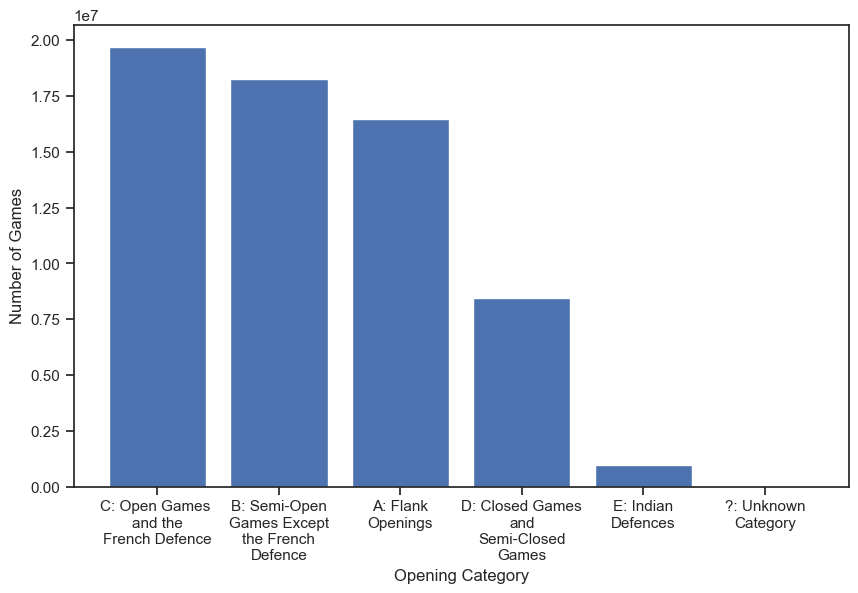
\includegraphics[width=0.8\textwidth]{Most Popular Openings by Category.png}
\end{figure}

We also counted the most popular openings by category in figure \ref{fig:mostPopularOpeningsByCategory}, as this is represented by the ECO column provided in the Lichess PGN data. ECO (Encyclopedia of Chess Openings) is a classification of chess openings based on the first few moves of the game. Editors who mostly consist of chess grandmasters select critical opening lines and assign them a code \cite{matanovic1971classification}. The ECO system consists of five categories, A to E, each of which represent a category of opening. Within each category, there are further subcategories to group openings more explicitly. For example, a game with an ECO code of A41 means that the opening is a flank opening as it is in the A category, and the 41 means that the opening was the Queen's Pawn Game. The ECO system is not perfect as it does not include all openings (as demonstrated by the 32,799 games with the unknown category in figure \ref{fig:mostPopularOpeningsByCategory}), but it is useful to analyse opening trends.

Figure \ref{fig:mostPopularOpeningsByCategory} shows that the most popular category of openings are open games and semi-open games, whereas the Indian defences and closed games are the least popular. This makes sense for the general population of games -- the ideas behind these openings are simple and straightforward, as they focus on controlling the centre and developing pieces quickly. However, we see that the pattern is different for players rated 2000 and above -- semi-open games and flank openings are more popular than open games in this category (shown in figure \ref{fig:mostPopularOpeningsByCategoryRated2000Plus} from the appendices). At higher rated games, players often prefer to play more complex and dynamic openings that enable opportunities to create imbalances in the position and therefore gain an advantage at an earlier stage of the game.

\subsection{Most Popular Base Openings}
\begin{figure}[H]
    \centering
    \caption{Most Popular Base Openings on Lichess in 2022}
    \label{fig:mostPopularOpenings}
    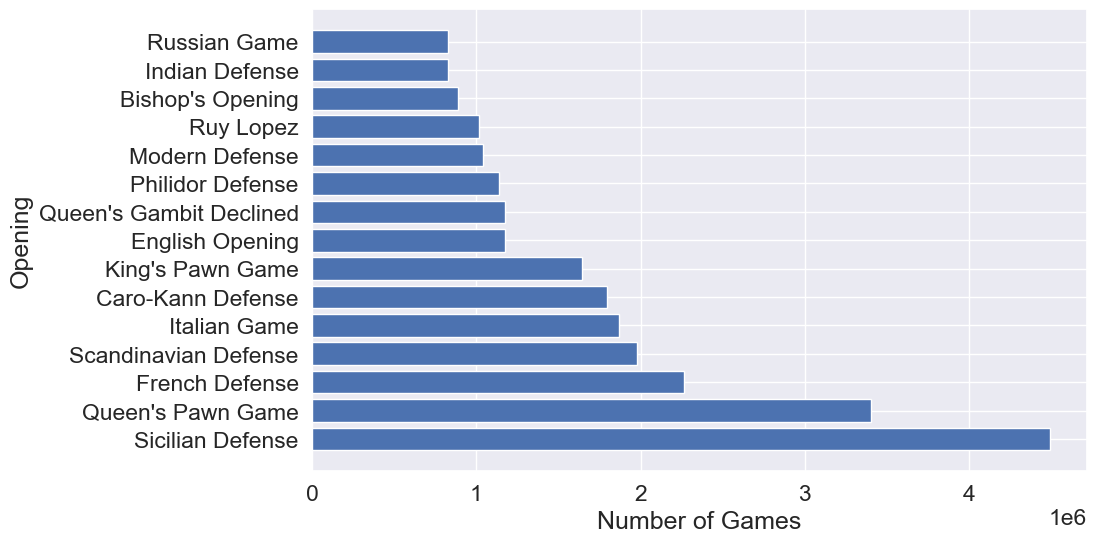
\includegraphics[width=0.8\textwidth]{Most Popular Base Openings.png}
\end{figure}

The data set also includes a column for the specific opening detected in each game based on Lichess' opening detection. We grouped openings that were different variations of each other into base openings to get a more accurate representation -- figure \ref{fig:examplesOfChessOpenings} from the appendices contains examples of base openings on the chess board. The top 15 most popular base openings account for 61.79\% of all games in our data set. Figure \ref{fig:mostPopularOpenings} shows that the most popular openings are the Sicilian Defence and the Queen's Pawn Game by a significant margin. The Sicilian Defence is the most well-studied response to White moving the king's pawn forward by two, which could explain why it is the most popular opening. However, the Queen's Pawn Game is slightly misleading, as it describes any opening beginning with White moving the queen's pawn where they do not play the Queen's Gambit and therefore encompasses a large number of openings such as the London System which are not labelled separately.

Delving deeper into the data, we found that the most popular base openings varied by rating groups. The top players rated 2000 and above strongly preferred the Sicilian Defense compared to other openings (shown in figure \ref{fig:mostPopularOpeningsRated2000Plus} from the appendices). This may be because the Sicilian Defense is a complex opening that requires a lot of preparation due to the number of variations, and it is unanimously accepted as the best response to White opening with the king's pawn. Conversely, the Sicilian Defense becomes much less popular for players rated 1200 and below for the same reasons. Figure \ref{fig:mostPopularOpeningsRated1200Minus} from the appendices shows that the two most popular base openings for this group are the Queen's Pawn Game and the King's Pawn Game, which represent generic openings starting with the queen's pawn and the king's pawn respectively -- this is likely because they are simple and easy for beginners to play.

\section{Results and Evaluation}

\section{Conclusion}

\subsection{Limitations and Future Work}

\bibliography{main.bib}
\bibliographystyle{ieeetr.bst}

\newpage
\begin{appendices}

\section{Additional Outputs}
\begin{figure}[H]
    \centering
    \caption{Effect of Higher Rating on White Win Rate on Lichess in 2022}
    \label{fig:effectOfHigherRatingOnWhiteWinRate}
    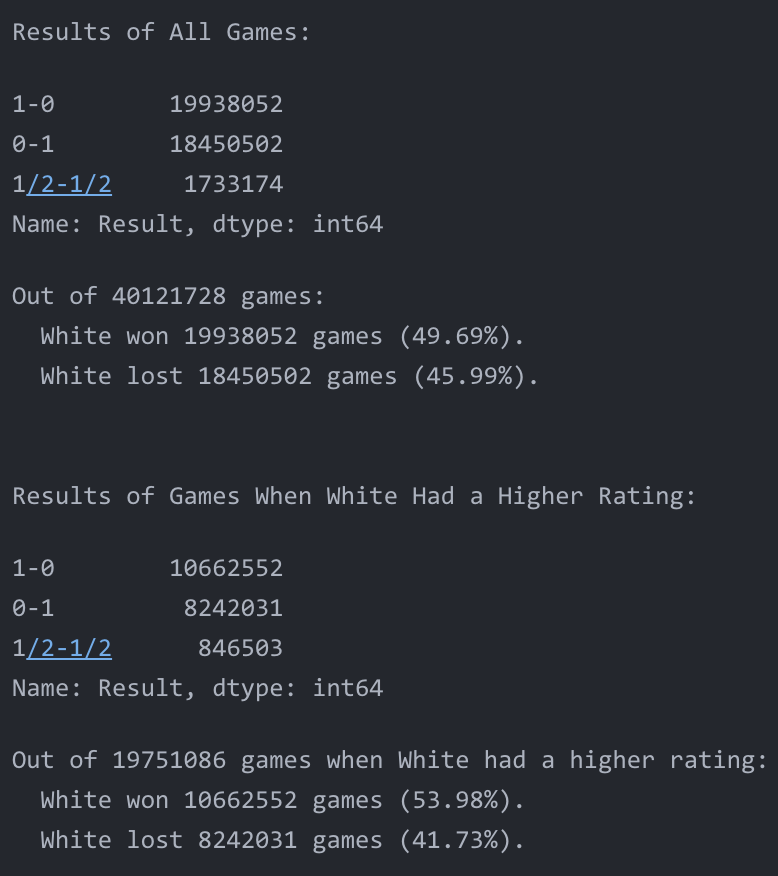
\includegraphics[width=0.5\textwidth]{Effect of Higher Rating on White Win Rate.png}
\end{figure}

\section{Additional Plots}
\begin{figure}[H]
    \centering
    \caption{Distribution of Absolute Rating Difference on Lichess in 2022}
    \label{fig:distributionOfAbsoluteRatingDifference}
    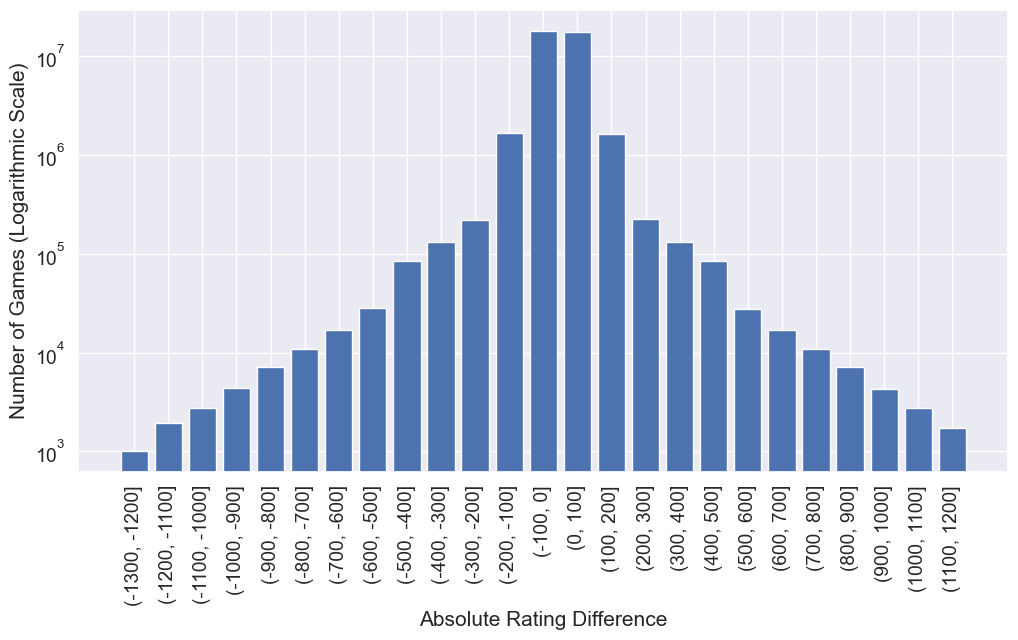
\includegraphics[width=0.8\textwidth]{Distribution of Absolute Rating Difference.png}
\end{figure}

\begin{figure}[H]
    \centering
    \caption{Distribution of Relative Rating Difference on Lichess in 2022}
    \label{fig:distributionOfRelativeRatingDifference}
    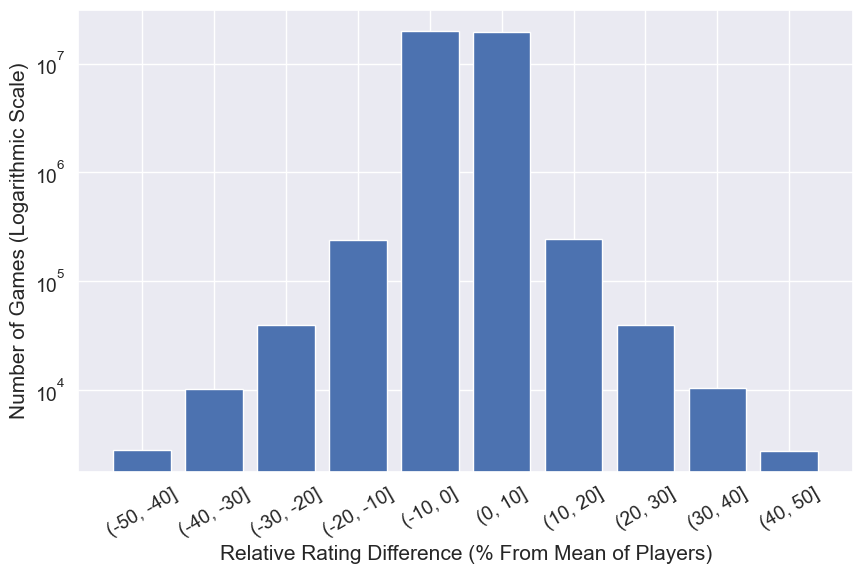
\includegraphics[width=0.8\textwidth]{Distribution of Relative Rating Difference.png}
\end{figure}

\begin{figure}[H]
    \centering
    \caption{Mean White Win Rate for Each EloDiff Bin}
    \label{fig:meanWhiteWinRateForEachEloDiffBin}
    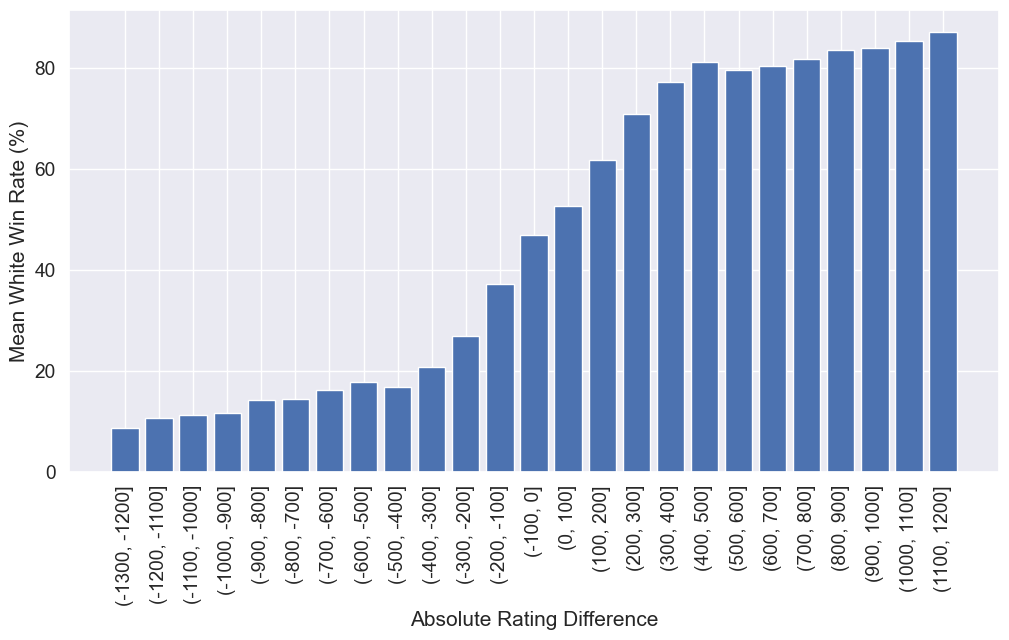
\includegraphics[width=0.8\textwidth]{Mean White Win Rate for Each EloDiff Bin.png}
\end{figure}

\begin{figure}[H]
    \centering
    \caption{Most Popular Openings by Category on Lichess in 2022 (Rated 2000 and Above)}
    \label{fig:mostPopularOpeningsByCategoryRated2000Plus}
    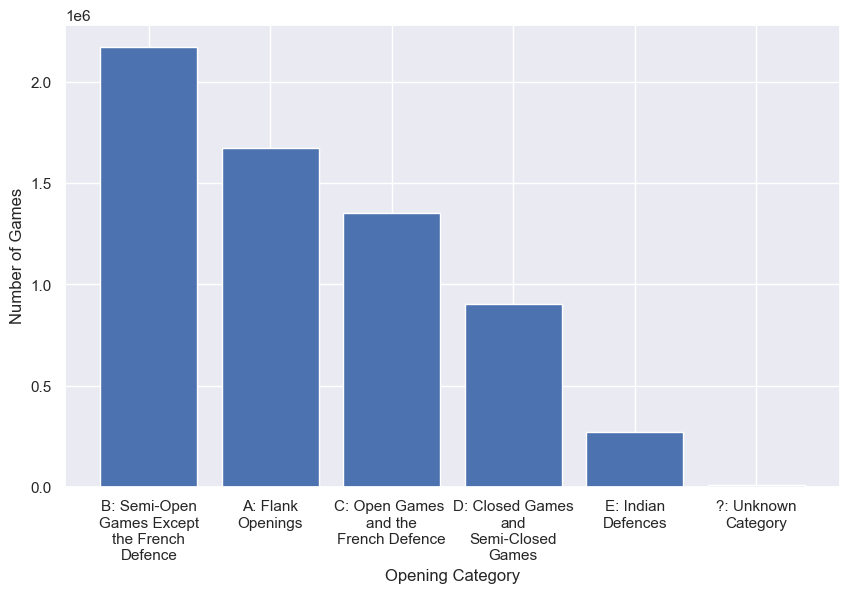
\includegraphics[width=0.8\textwidth]{Most Popular Openings by Category (Rated 2000+).png}
\end{figure}

\begin{figure}[H]
    \centering
    \caption{Most Popular Base Openings on Lichess in 2022 (Rated 2000 and Above)}
    \label{fig:mostPopularOpeningsRated2000Plus}
    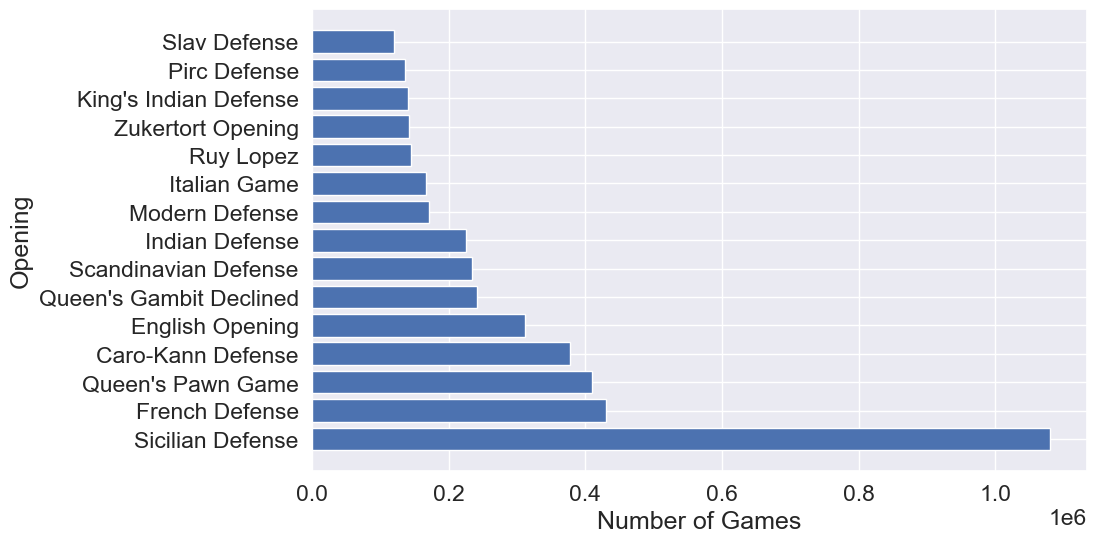
\includegraphics[width=0.8\textwidth]{Most Popular Base Openings (Rated 2000+).png}
\end{figure}

\begin{figure}[H]
    \centering
    \caption{Most Popular Base Openings on Lichess in 2022 (Rated 1200 and Below)}
    \label{fig:mostPopularOpeningsRated1200Minus}
    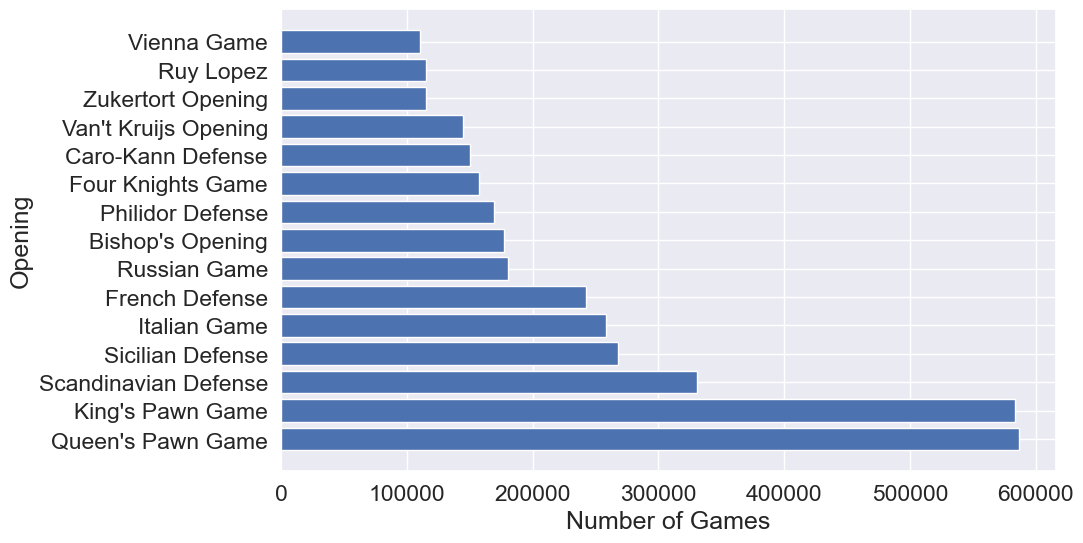
\includegraphics[width=0.8\textwidth]{Most Popular Base Openings (Rated 1200-).png}
\end{figure}

\section{Examples}
\begin{figure}[H]
    \centering
    \caption{Examples of Chess Openings}
    \label{fig:examplesOfChessOpenings}
    \begin{subfigure}{0.45\textwidth}
        \centering
        \caption{Sicilian Defence}
        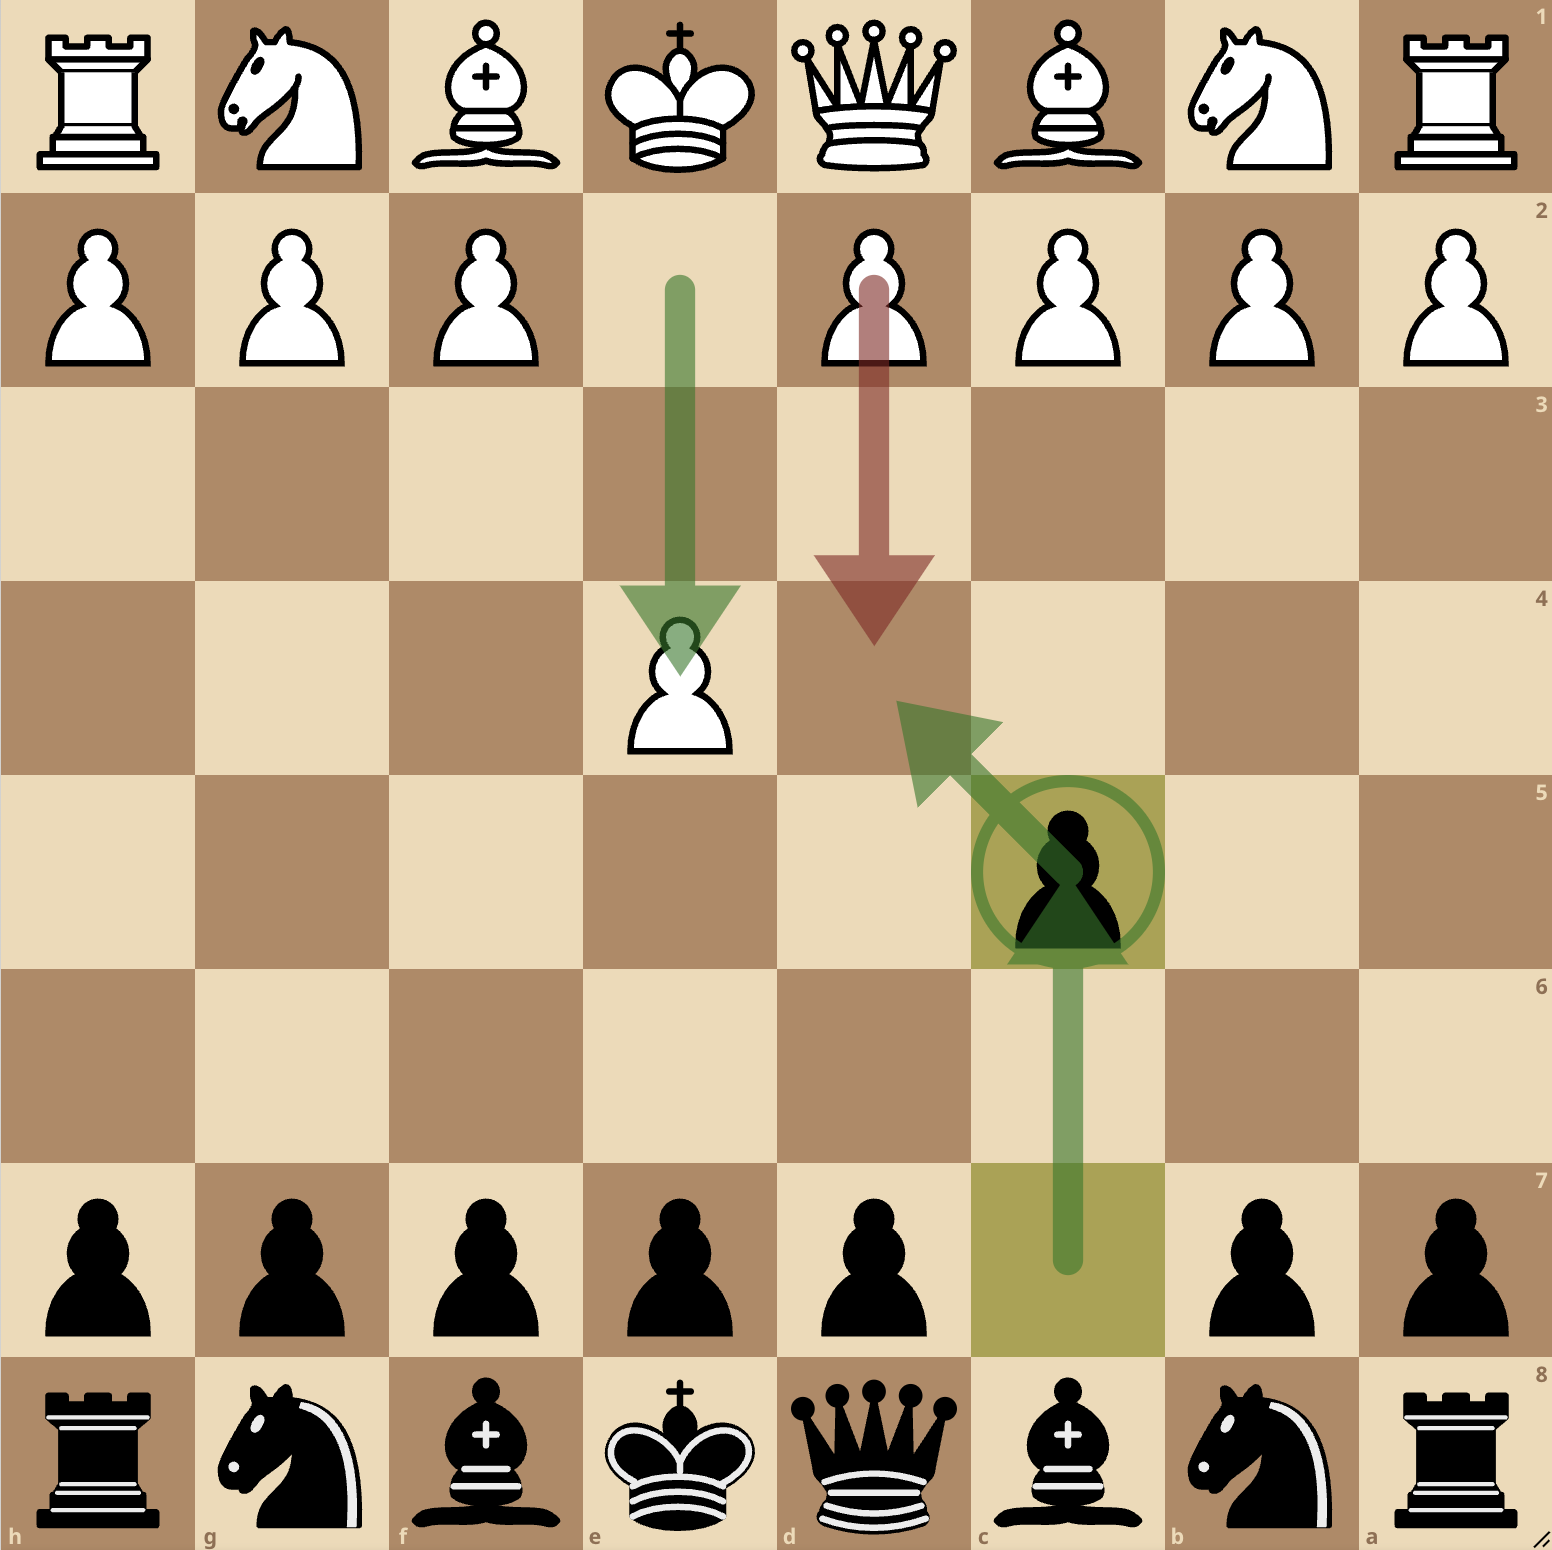
\includegraphics[width=\textwidth]{Example of Sicilian Defence.png}
    \end{subfigure}
    \hfill
    \begin{subfigure}{0.45\textwidth}
        \centering
        \caption{Queen's Gambit}
        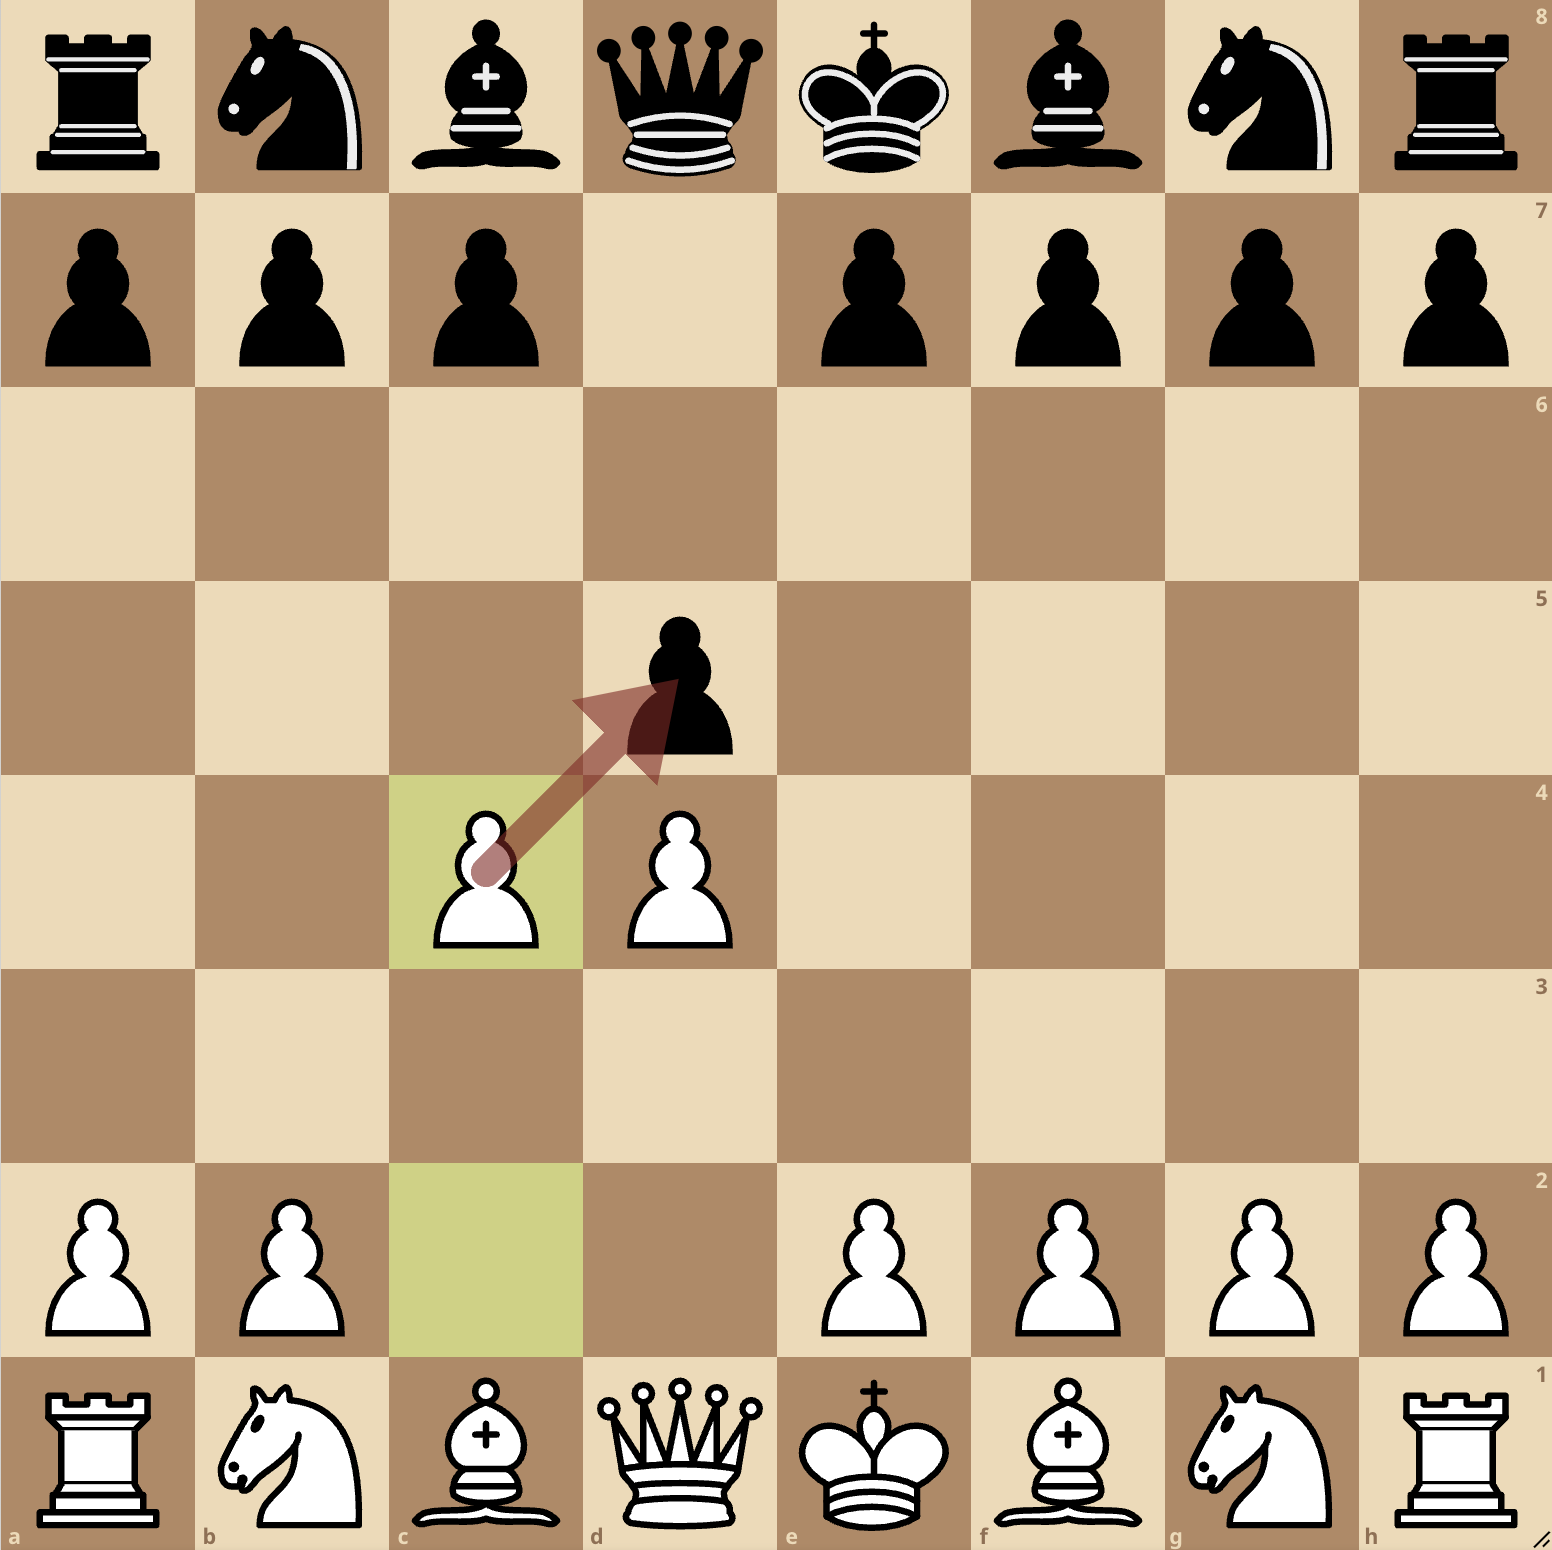
\includegraphics[width=\textwidth]{Example of Queen's Gambit.png}
    \end{subfigure}
\end{figure}

\end{appendices}

\end{document}